% !TEX root = mythesis.tex

%==============================================================================
\chapter{The \tZqsec production}
\label{sec:tZq}
%==============================================================================

High energy proton-proton collisions at the LHC enable
multiple processes to take place. The process of interest for this analysis 
is the electroweak production of the \Ptop-quark and the 
\PZ-boson. The LO $t$-channel Feynman diagrams are shown in \cref{fig:tZqfeyn} where
a \PZ-boson can be radiated from any one of the incoming or outgoing quarks (\cref{fig:tZqfeyna})
or from the exchanged \PW-boson (\cref{fig:tZqfeynb}). In addition to these
resonant contributions, there is also a small non-resonant contribution 
in the form of $tl^+l^-q$ (\cref{fig:tZqfeync}) which is also accounted for. 
In this analysis, this process
is referred to as the \tZq production. 

\begin{figure}[htbp]
    \centering
    % \begin{subfigure}{0.35\figwidth}
    %   \centering
    %      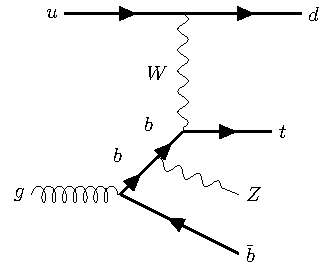
\includegraphics[width=\textwidth]{tZq_Zfromb.pdf}
    %      \caption{}
    %      \label{fig:tZqfeyna}
    % \end{subfigure}
    % \qquad
    \begin{subfigure}{0.35\figwidth}
      \centering
      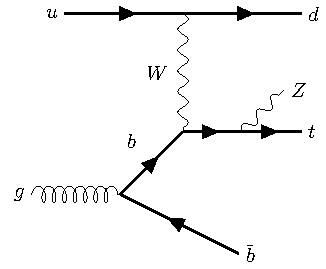
\includegraphics[width=\textwidth]{tZq_Zfromtop.pdf}
      \caption{}
      \label{fig:tZqfeyna}
    \end{subfigure}
    \begin{subfigure}{0.35\figwidth}
      \centering
      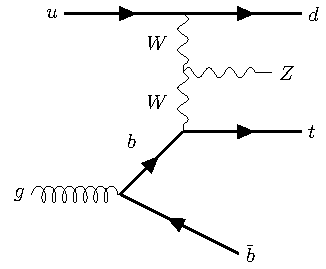
\includegraphics[width=\textwidth]{tZq_ZfromWW.pdf}
      \caption{}
      \label{fig:tZqfeynb}
    \end{subfigure}
  
  
  \medskip
  
  
  \begin{subfigure}{0.35\figwidth}
      \centering
      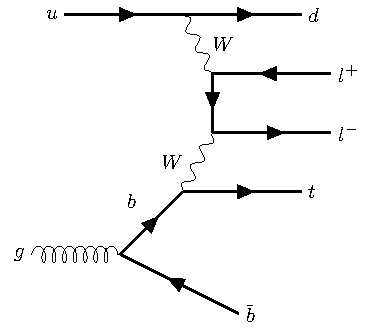
\includegraphics[width=\textwidth]{tZq_nonres.pdf}
      \caption{}
         \label{fig:tZqfeync}
    \end{subfigure}
    % \begin{subfigure}{0.35\figwidth}
    %   \centering
    %   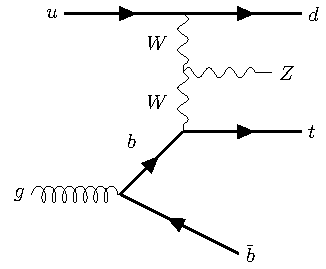
\includegraphics[width=\textwidth]{tZq_ZfromWW.pdf}
    %   \caption{}
    %      \label{fig:tZqfeyne}
    % \end{subfigure}
    % \begin{subfigure}{0.35\figwidth}
    %     \centering
    %     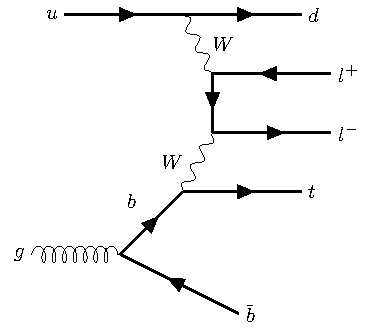
\includegraphics[width=\textwidth]{tZq_nonres.pdf}
    %     \caption{}
    %      \label{fig:tZqfeynf}
    %   \end{subfigure}
  
  \caption[Feynman diagrams at LO for the \tZq-production]{Feynman diagrams at 
  LO for the \tZq-production. The \PZ is radiated either from one of the
  quarks or from the exchanged W boson. }
  \label{fig:tZqfeyn}
  \end{figure}

The \tZq production is an interesting process to study because it probes the coupling
of two fermions and the coupling of a fermion to a boson in the same interaction. Moreover, 
it can provide a solid basis to study similar processes such as the $tHq$ process. 

In order to study this process, one has to note 
that the particles involved in this production are quite heavy and therefore,
the only way to spot them is from their reconstructed decay products. 
Conventionally, the possible final states are divided into several \textit{channels}
based on certain combinations of leptons and jets. This analysis focuses on
the so-called trilepton channel.

\section{The \tZqsec Trilepton Channel}
As the name suggests, the trilepton decay channel of the \tZq production 
contains final states with three charged leptons, as shown in \cref{fig:tZqtrilep}. The
\Ptop-quark decays almost exclusively into \Pbottom\PW and the corresponding \PW decays into a charged lepton and
a neutrino. The \PZ-boson decays into opposite sign same flavour leptons. The probability for
\PZ decaying into leptons is equal across the three lepton families (\Pelectron,\Pmu,\Ptau) due to 
lepton universality. This analysis accounts for \PZ decays resulting into \Pelectron, \Pmu and 
leptonically decaying \Ptau \footnote{\Ptau is a heavy particle and hence, can be observed only via its decays}.   

Although the trilepton final state has a small branching ratio, it has a very clean signature
due to the three lepton requirement. In addition, three lepton final state is quite difficult
to mimic by backgrounds. This is the reason to choose this final state for studying \tZq process.
For this analysis, the trilepton final state is referred to as the signal.

\begin{figure}
  \centering
      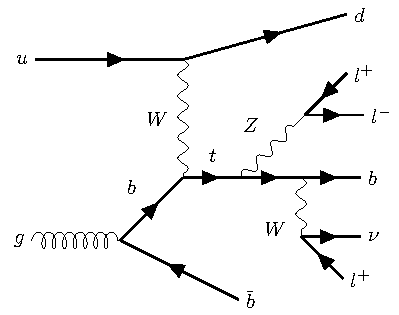
\includegraphics[width=0.45\textwidth]{tZq_Zfromtop_decay.pdf}
      \caption{The \tZq trilepton final state}
         \label{fig:tZqtrilep}
\end{figure}

The next task is to reconstruct this final state from the detector data or in other words, find
possible occurrences of this final state within the collision events. In order to achieve that,
certain requirements are defined in favour of the signal events. The collection of these requirements
is called event selection. For this analysis, the primary event selection is discussed below and
summarised in \cref{tab:selection:srcr}.

\begin{itemize}
  \item \textbf{Leptons}
    \begin{itemize}
      \item Exactly three leptons (\Pelectron or \Pmu), 
      \Ptau is considered if it decays into leptons. These leptons are 
      sorted by their \pT which is required to be at least 27,15 and 10 GeV, respectively.
      
      \item At least 1 Opposite Sign Same Flavour (OSSF) lepton pair with a minimum
      difference between its invariant mass ($m_{ll}$) and $m_Z$. This is to identify 
      which out of the selected leptons originate from \PZ.

      \item A cut on minimum accepted invariant mass, in order to suppress backgrounds 
      not containing a \PZ.

      \item A cut on the transverse mass of the \PW-boson is applied to account for the missing
      transverse energy. 
  \end{itemize}
  \item \textbf{Jets}
  \begin{itemize}
    \item Number of jets are required to be between 2 and 5, with \pT more than \qty{25}{GeV}
    and $|\eta|$ more than 4.5.
    \item Number of \Pbottom-jets are required to be 1 or 2, reconstructed at $85\%$ working 
    point with $|\eta|$ more than 2.5. Events with 2 jets, both \Pbottom-tagged are not considered.
  \end{itemize}


\end{itemize}

\begin{table}[!htbp]
    \footnotesize
    \caption{Event selection}
    \label{tab:selection:srcr}
    \renewcommand{\arraystretch}{1.3}
    \centering
    \begin{tabular}{lccc}
        \toprule
        Variable & \multicolumn{3}{c}{Preselection}\\
        \midrule
        $N_\ell~\left(\ell=e,\mu\right)$ & \multicolumn{3}{c}{$=3$}\\
        & \multicolumn{3}{c}{$\ge 1$ OSSF lepton pair}\\
        $\pT\left(\ell_1,\ell_2,\ell_3\right)$ & \multicolumn{3}{c}{$>$ 27,~15, \qty{10}{\GeV}}\\
        $\min(m_{\ell\ell})$ & \multicolumn{3}{c}{$>$ \qty{20}{\GeV}} \\
        $|m_{\ell\ell} - m_{Z}|$ & \multicolumn{3}{c}{$<$ \qty{10}{\GeV}} \\
        \mtw & \multicolumn{3}{c}{$>$ \qty{30}{\GeV}} \\
        $N_\text{jets}\left(\pT>25~\mathrm{GeV}\right)$ & \multicolumn{3}{c}{2-5} \\
        $N_{b-\text{jets}} @ 85\%$ & \multicolumn{3}{c}{1-2 (no $2j2b$)} \\
        % & SR & \CRttZ & \CRVV \\
        % $N_\text{jets}\left(\pT>25~\mathrm{GeV}\right)$ & 2-5 & $\ge 6$ & 2-5 \\
        % $N_{b-\text{jets}} @ 85\%$ & 1-2 (no $2j2b$) & $\ge 1$ & 0 \\
        \bottomrule
    \end{tabular}
    \end{table}


It is important to note here that these requirements are chosen to 
maximise the probability of selecting signal events
but in reality there are background processes that mimic the \tZq signature
and therefore, contaminate the selected signal events. 

\section{Background processes}

The background processes for \tZq process can be classified according to the number of prompt (or real)
leptons in the final state. A lepton is labelled prompt if it originates from either a \Ptau or a 
massive boson. On the other hand, non-prompt or fake leptons are objects misidentified as leptons.
The source of non-prompt leptons can be bottom and charm hadron decays, meson decays, 
photon conversions or light jets creating lepton-like signatures. Backgrounds involving only prompt leptons
are \diboson, \ttX, \ttH and \tWZ while backgrounds involving non-prompt leptons are \Ptop{}\APtop,
\PZ+jets and \tW.

\subsection*{Backgrounds involving prompt leptons}

In the \diboson process, two massive bosons are produced which can be \PZ{}\PZ, \PW{}\PW or \PW{}\PZ,
as shown in \cref{fig:VVfeyn}. As per \cref{fig:VVfeyna}, the leptonic decay of bosons result 
into three prompt leptons which can pass the signal event selection if additional jets are also found.
For the \PZ{}\PZ scenario, as shown in \cref{fig:VVfeynb}, one of the leptons needs to fail the 
requirement for a prompt lepton or is not reconstructed. Due to this strong resemblance of the 
\diboson signature with the signal, it is the dominant background in the \tZq production. 

\begin{figure}[htbp]
  \centering
  \begin{subfigure}{0.45\figwidth}
    \centering
    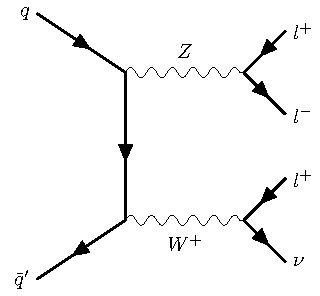
\includegraphics[width=\textwidth]{Feynman_WZ.pdf}
    \caption{}
    \label{fig:VVfeyna}
  \end{subfigure}
  \begin{subfigure}{0.45\figwidth}
    \centering
    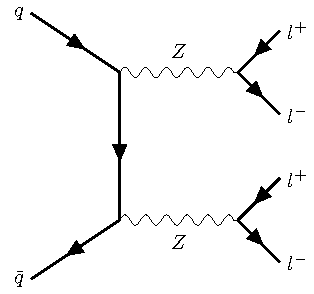
\includegraphics[width=\textwidth]{Feynman_ZZ.pdf}
    \caption{}
    \label{fig:VVfeynb}
  \end{subfigure}
  \caption[Feynman diagrams for \diboson backgrounds]{Feynman diagrams for the \diboson background}
  \label{fig:VVfeyn}
  \end{figure}

The \Ptop-quark pair production in association with a heavy boson (\PZ or \PW) can be an
important source of background. In particular, the \ttZ process, where the 
final state already includes a \PZ boson and a \Ptop quark, can produce a very 
similar signal-like signature. It is shown in \cref{fig:ttZ}. The \ttH contributes
less because of its small cross-section.

\begin{figure}
  \centering
      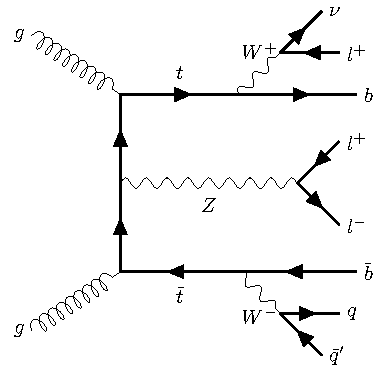
\includegraphics[width=0.45\textwidth]{Feynman_ttbarV.pdf}
      \caption{Feynman diagrams for the \ttZ background}
         \label{fig:ttZ}
\end{figure}

\subsection*{Backgrounds involving non-prompt leptons}

Backgrounds involving non-prompt or fake lepton are \Ptop-quark pair production 
and the production \PZ-boson with jets. 
As shown in \cref{fig:fakefeynb}, there are already two leptons
from the \PZ-boson. If the jets are light, they can be misidentified as leptons leading to 
a non-prompt lepton contribution.
In the \Ptop{}\APtop production, as shown in \cref{fig:fakefeynb}, if one of the \Pbottom-jet decays 
into a lepton, then it can satisfy the signal event selection.


\begin{figure}[htbp]
  \centering
  \begin{subfigure}{0.45\figwidth}
    \centering
    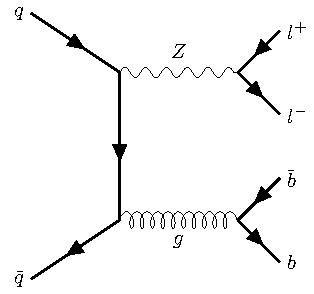
\includegraphics[width=\textwidth]{ZPlusJets_standalone.pdf}
    \caption{}
    \label{fig:fakefeyna}
  \end{subfigure}
  \begin{subfigure}{0.45\figwidth}
    \centering
    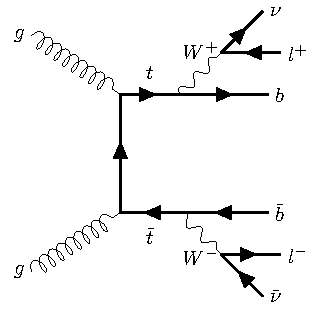
\includegraphics[width=\textwidth]{ttbar_standalone.pdf}
    \caption{}
    \label{fig:fakefeynb}
  \end{subfigure}
  \caption[Feynman diagrams for non-prompt lepton backgrounds]{Feynman diagrams for non-prompt lepton background}
  \label{fig:fakefeyn}
  \end{figure}